\documentclass[14pt]{extarticle}
\usepackage{fontspec}
\usepackage{polyglossia}
\usepackage{amsmath}
\usepackage{amssymb}
\usepackage{xcolor}
\usepackage{fancyhdr}
\usepackage{graphicx}
\usepackage{listings}
\usepackage[most]{tcolorbox}
% \usepackage{setspace}
\usepackage{pifont}
\usepackage{enumitem}
\usepackage{titlesec}
\usepackage[bottom]{footmisc}
\usepackage{titling}
\usepackage{minted}
\usepackage{etoolbox}
\usepackage{array}
\usepackage{extsizes}
\usepackage{float}
\usepackage{booktabs}
\usepackage{hyperref}
\usepackage[onehalfspacing]{setspace}
\usepackage[a4paper, top=2.7cm, bottom=2.7cm, left=2.5cm, right=2.5cm, headheight=1.5cm, headsep=0.5cm]{geometry}
\usepackage{tikz}

\usetikzlibrary{automata, positioning, arrows.meta, arrows}

\newfontfamily\emoji{Segoe UI Emoji}

\pagestyle{fancy}

\setmainlanguage[numerals=western]{arabic}
\setotherlanguage{english}
% \newfontfamily\arabicfont[Script=Arabic]{Amiri}
\newfontfamily\arabicfont[Script=Arabic]{Calibri}
\newfontfamily\arabicfonttt[Script=Arabic]{Courier New}

\lstset{
  language=[Sharp]C,
  numbers=left,
  stepnumber=1,
  numbersep=8pt,
  frame=single,
  basicstyle=\ttfamily\small,
  keywordstyle=\color{blue},
  stringstyle=\color{red},
  commentstyle=\color{green!50!black}
}

\newif\ifdetailed
\ifdefined\setdetailed
  \setdetailed
\fi

\newif\ifwithsols
\ifdefined\setwithsols
  \setwithsols
\fi

% unified tcolorboxes for articles
\tcbset{colback=white, colframe=black, fonttitle=\bfseries, boxrule=0.8pt}
\newtcolorbox{boxDef}[1][]{colback=blue!5!white,colframe=blue!75!black,
  title={{\emoji📘} تعريف\ifx\\#1\\\else ~#1\fi :}}
\newtcolorbox{boxExercise}[1][]{colback=cyan!5!white,colframe=cyan!70!black,
  title={{\emoji🧩} تمرين\ifx\\#1\\\else ~#1\fi :}}
\newtcolorbox{boxExample}[1][]{colback=yellow!5!white,colframe=orange!90!black,
  title={{\emoji📝} مثال\ifx\\#1\\\else ~#1\fi :}}
\newtcolorbox{boxNote}[1][]{colback=gray!10!white,colframe=black,
  title={{\emoji✨} ملاحظة\ifx\\#1\\\else ~#1\fi :}}
\newtcolorbox{boxAttention}[1][]{colback=magenta!10!white,colframe=magenta!80!black,
  title={{\emoji🔔} تنبيه\ifx\\#1\\\else ~#1\fi :}}
\newtcolorbox{boxWarning}[1][]{colback=red!5!white,colframe=red!75!black,
  title={{\emoji⚡} ملاحظة هامة\ifx\\#1\\\else ~#1\fi :}}
\newtcolorbox{boxSolution}[1][]{colback=green!5!white,colframe=green!60!black,
  title={{\emoji✅} حل\ifx\\#1\\\else ~#1\fi :}}
\newtcolorbox{boxSymbol}[1][]{colback=purple!5!white,colframe=purple!70!black,
  title={{\emoji🔣} رمز\ifx\\#1\\\else ~#1\fi :}}
\newtcolorbox{boxHint}[1][]{colback=teal!5!white,colframe=teal!60!black,
  title={{\emoji💡} تلميح\ifx\\#1\\\else ~#1\fi :}}


\tcbset{simplecode/.style={ colback=gray!5, colframe=black!50, boxrule=0.4pt, arc=2pt, left=4pt,right=4pt,top=4pt,bottom=4pt}}
\newenvironment{boxCode}{\begin{tcolorbox}[simplecode]}{\end{tcolorbox}}

\newcolumntype{C}[1]{>{\centering\arraybackslash}p{#1}}

% redefine spaces after titles
\makeatletter
\renewcommand{\@maketitle}{%
  \begin{center}
    {\huge \bfseries \@title \par}%
    \vskip 0.2em % space between title and author
    {\large \@author \par}%
    % \vskip 0.2em % space between author and date
    % {\normalsize \@date \par}%
  \end{center}
}
\makeatother

\fancyhf{} % clear default
\fancypagestyle{plain}{
  \fancyhf{}
  \fancyhead[L]{مدرسة التسامح الشاملة}
  % \fancyhead[L]{
\includegraphics[height=1cm]{../../../images/logoTasamoh.png}}
  \fancyhead[R]{الأستاذ محمود اغبارية}
  \fancyfoot[C]{\thepage}
}

\fancyhead[L]{مدرسة التسامح الشاملة}
\fancyhead[R]{الأستاذ محمود اغبارية}
\fancyfoot[C]{\thepage}
% \date{\today}

\setcounter{tocdepth}{3} % only section subsection and subsubsection in TOC

\newcommand{\importpdfpage}[2]{%
    \thispagestyle{empty}
    \newgeometry{left=0cm,right=0cm,top=0cm,bottom=0cm}
    \includegraphics[page=#2,width=0.95\paperwidth,height=0.95\paperheight,keepaspectratio]{#1}
    \restoregeometry
}

\newcommand{\insertFullImg}[1]{%
    \noindent
    \makebox[\textwidth][c]{
        \includegraphics[width=0.9\paperwidth,keepaspectratio]{#1}%
    }%
}%

% ----------------------


% \begin{document}

% \maketitle

% % \clearpage  % start TOC on a new page
% % \renewcommand{\contentsname}{جدول المحتويات}
% % \tableofcontents
% % \clearpage

% \part*{part 1} % the * prevents numbering
% \section*{مقدمة}
% \subsection*{مثال رياضي}
% \subsubsection*{مثال فرعي}
% \paragraph*{ paragraph 1}
% \subparagraph*{sub paragraph 1}

% \ifdetailed
% \begin{english}
% \begin{minted}{csharp}
% // C# Example
% \end{minted}
% \end{english}
% \fi

% OLD WAY
% \ifdetailed
% \begin{english}
% \begin{lstlisting}
% // C# Example
% \end{lstlisting}
% \end{english}
% \fi

% % 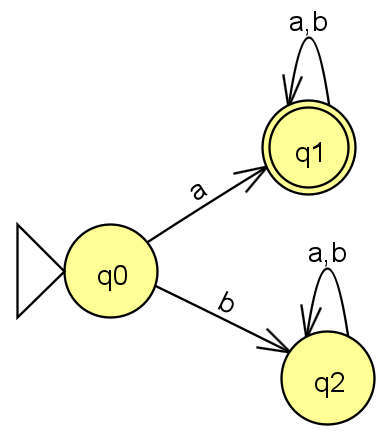
\includegraphics[width=0.2\textwidth]{../../../images/DFAs/ex1_q1.png}



% \vspace{3cm}
% \begin{flushleft}
% أرجو لكم وقتًا ممتعًا.

% الأستاذ محمود اغبارية.
% \end{flushleft}


% \end{document}


\ifwithsols
\title{حل وظيفة: الفئات والكائنات 2}
\else
\title{وظيفة: الفئات والكائنات 2}
\fi

\begin{document}

\maketitle
\thispagestyle{fancy}

\begin{enumerate}[itemsep=2em]

% ======================================================
% سؤال 1 - فئة TrafficLight
% ======================================================
\item
سنبني فئة تمثل إشارة مرور.

\begin{enumerate}[itemsep=1em]
    \item أنشئ فئة باسم \textenglish{TrafficLight} تحتوي على الحقول الخاصة (\textenglish{private}) التالية:
    \begin{itemize}[itemsep=1pt]
        \item \textenglish{string Location} — موقع الإشارة
        \item \textenglish{string Color} — اللون الحالي للإشارة، تُبتدأ قيمته تلقائيًا بـ \textenglish{"Red"} في العملية البنّاءة بغضّ النظر عن أي معطى
        \item \textenglish{int CycleCount} — عدد دورات التبديل الكاملة التي مرّت، يُبتدأ بـ \textenglish{0} في العملية البنّاءة
    \end{itemize}
    أضف عملية بنّاءة تستقبل موقع الإشارة فقط.

    \item أضف عمليات \textenglish{GetLocation()}، و\textenglish{GetColor()}، و\textenglish{GetCycleCount()}.

    \item أضف عملية \textenglish{string Advance()} تُبدّل لون الإشارة إلى اللون التالي وفق الترتيب:\\
    \textenglish{Red} $\to$ \textenglish{Green} $\to$ \textenglish{Yellow} $\to$ \textenglish{Red} $\to$ \ldots\\
    في كل مرة يعود اللون إلى \textenglish{"Red"}، تزيد قيمة \textenglish{CycleCount} بمقدار 1.\\
    تعيد العملية اللون الجديد بعد التبديل.

    \item أضف عملية \textenglish{bool IsGo()} تعيد \textenglish{true} إذا كان اللون الحالي \textenglish{"Green"}.

    \item أضف عملية \textenglish{void Print()} تطبع الإشارة بالتنسيق التالي:\\
    \textenglish{[Main St.] Color: Green | Cycles: 2}

    \item في الدالة الرئيسية \textenglish{Main}، اكتب الأوامر التالية بالترتيب لاختبار الفئة:
    \begin{enumerate}[itemsep=1pt, label=(\roman*)]
        \item عرّف كائنًا يمثل إشارة مرور في موقع \textenglish{"Main St."}، واطبعها باستخدام \textenglish{Print()}.
        \item استدعِ الدالة \textenglish{Advance()} ثلاث مرات متتالية، واطبع القيمة التي تعيدها كل مرة.
        \item استدعِ \textenglish{IsGo()} واطبع القيمة التي تعيدها، ثم اطبع حالة الإشارة باستخدام \textenglish{Print()}.
        \item استدعِ \textenglish{Advance()} مرتين إضافيتين، واطبع القيمة التي تعيدها كل مرة، ثم اطبع حالة الإشارة باستخدام \textenglish{Print()}.
    \end{enumerate}
\end{enumerate}

\ifwithsols
{\small
\begin{boxSolution}
\begin{english}
\begin{minted}{csharp}
class TrafficLight
{
    private string Location;
    private string Color;
    private int CycleCount;

    public TrafficLight(string location)
    {
        this.Location   = location;
        this.Color      = "Red";
        this.CycleCount = 0;
    }

    public string GetLocation()  { return Location;   }
    public string GetColor()     { return Color;      }
    public int    GetCycleCount(){ return CycleCount; }

    public string Advance()
    {
        if (Color == "Red")
            Color = "Green";
        else if (Color == "Green")
            Color = "Yellow";
        else
        {
            Color = "Red";
            CycleCount++;
        }
        return Color;
    }

    public bool IsGo()
    {
        return Color == "Green";
    }

    public void Print()
    {
        Console.WriteLine($"[{Location}] Color: {Color} | Cycles: {CycleCount}");
    }
}
\end{minted}
\end{english}
\end{boxSolution}
\begin{boxSolution}
\begin{english}
\begin{minted}{csharp}
public static void Main()
{
    TrafficLight tl = new TrafficLight("Main St.");
    tl.Print();

    Console.WriteLine(tl.Advance()); // Green
    Console.WriteLine(tl.Advance()); // Yellow
    Console.WriteLine(tl.Advance()); // Red  -> CycleCount becomes 1

    Console.WriteLine("IsGo: " + tl.IsGo());
    tl.Print();

    Console.WriteLine(tl.Advance()); // Green
    Console.WriteLine(tl.Advance()); // Yellow
    tl.Print();
}
\end{minted}
\end{english}
\end{boxSolution}
}
\fi
\clearpage

% ======================================================
% سؤال 2 - فئة Scoreboard
% ======================================================
\item
سنبني فئة تمثل لوحة نتائج لمباراة رياضية.

\begin{enumerate}[itemsep=1em]
    \item أنشئ فئة باسم \textenglish{Scoreboard} تحتوي على الحقول الخاصة (\textenglish{private}) التالية:
    \begin{itemize}[itemsep=1pt]
        \item \textenglish{string TeamA} — اسم الفريق الأول
        \item \textenglish{string TeamB} — اسم الفريق الثاني
        \item \textenglish{int ScoreA} — نقاط الفريق الأول، تُبتدأ بـ \textenglish{0} في العملية البنّاءة
        \item \textenglish{int ScoreB} — نقاط الفريق الثاني، تُبتدأ بـ \textenglish{0} في العملية البنّاءة
    \end{itemize}
    أضف عملية بنّاءة تستقبل أسماء الفريقين فقط.

    \item أضف عمليات \textenglish{GetScoreA()}، و\textenglish{GetScoreB()}.

    \item أضف عملية \textenglish{string ScoreGoal(string team)} تُسجّل هدفًا للفريق المُمرَّر (يجب أن يساوي اسم أحد الفريقين، وإلا لا تفعل شيئًا).\\
    تزيد نقاط الفريق بمقدار 1>\\
    تعيد العملية اسم الفريق الذي يتصدر النتيجة بعد الهدف. إذا تعادل الفريقان، تعيد \textenglish{"Draw"}.

    \item أضف عملية \textenglish{int GetDifference()} تعيد الفارق المطلق بين نقاط الفريقين\\
    (أي \textenglish{|ScoreA - ScoreB|}).

    \item أضف عملية \textenglish{void Print()} تطبع النتيجة بالتنسيق التالي:\\
    \textenglish{Haifa 3 - 1 Nazareth | Total Goals: 4}

    \item في الدالة الرئيسية \textenglish{Main}، اكتب الأوامر التالية بالترتيب لاختبار الفئة:
    \begin{enumerate}[itemsep=1pt, label=(\roman*)]
        \item عرّف كائنًا يمثل مباراة بين فريقي \textenglish{"Haifa"} و\textenglish{"Nazareth"}، واطبع الحالة الابتدائية.
        \item سجّل هدفًا لـ\textenglish{"Haifa"}. احفظ القيمة التي تعيدها العملية واطبعها، ثم اطبع النتيجة.
        \item سجّل هدفًا لـ\textenglish{"Nazareth"}. احفظ القيمة التي تعيدها العملية واطبعها، ثم اطبع النتيجة.
        \item سجّل هدفين إضافيين لـ\textenglish{"Haifa"} (كل هدف باستدعاء منفصل). بعد كل هدف احفظ القيمة التي تعيدها العملية واطبعها. في النهاية اطبع النتيجة الكاملة والفارق باستخدام \textenglish{GetDifference()}.
    \end{enumerate}
\end{enumerate}

\ifwithsols
{\small
\begin{boxSolution}
\begin{english}
\begin{minted}{csharp}
class Scoreboard
{
    private string TeamA;
    private string TeamB;
    private int ScoreA;
    private int ScoreB;

    public Scoreboard(string teamA, string teamB)
    {
        this.TeamA      = teamA;
        this.TeamB      = teamB;
        this.ScoreA     = 0;
        this.ScoreB     = 0;
    }

    public int GetScoreA()     { return ScoreA;     }
    public int GetScoreB()     { return ScoreB;     }

    public string ScoreGoal(string team)
    {
        if (team == TeamA)
            ScoreA++;
        else if (team == TeamB)
            ScoreB++;
        else
            return "";

        if (ScoreA > ScoreB)
            return TeamA;
        else if (ScoreB > ScoreA)
            return TeamB;
        else
            return "Draw";
    }

    public int GetDifference()
    {
        int diff = ScoreA - ScoreB;
        if (diff < 0)
            return -diff;
        return diff;
    }

    public void Print()
    {
        Console.WriteLine(
            $"{TeamA} {ScoreA} - {ScoreB} {TeamB} | Total Goals: {ScoreA + ScoreB}"
        );
    }
}
\end{minted}
\end{english}
\end{boxSolution}
\begin{boxSolution}
\begin{english}
\begin{minted}{csharp}
public static void Main()
{
    Scoreboard sb = new Scoreboard("Haifa", "Nazareth");
    sb.Print();

    string leader1 = sb.ScoreGoal("Haifa");
    Console.WriteLine("Leader: " + leader1);
    sb.Print();

    string leader2 = sb.ScoreGoal("Nazareth");
    Console.WriteLine("Leader: " + leader2);
    sb.Print();

    string leader3 = sb.ScoreGoal("Haifa");
    Console.WriteLine("Leader: " + leader3);

    string leader4 = sb.ScoreGoal("Haifa");
    Console.WriteLine("Leader: " + leader4);

    sb.Print();
    Console.WriteLine("Difference: " + sb.GetDifference());
}
\end{minted}
\end{english}
\end{boxSolution}
}
\fi
\clearpage


% % ======================================================
% % سؤال 3 - فئة WordTracker
% % ======================================================
% \item
% سنبني فئة تتبّع تكرار كلمة معيّنة في نصوص يُدخلها المستخدم.

% \begin{enumerate}[itemsep=1em]
%     \item أنشئ فئة باسم \textenglish{WordTracker} تحتوي على الحقول الخاصة (\textenglish{private}) التالية:
%     \begin{itemize}[itemsep=1pt]
%         \item \textenglish{string TargetWord} — الكلمة المستهدفة للبحث (تُستقبل من العملية البنّاءة)
%         \item \textenglish{int TotalCount} — العدد الإجمالي لتكرارات الكلمة المستهدفة في جميع النصوص المُمرَّرة، يُبتدأ بـ \textenglish{0}
%         \item \textenglish{int TextsChecked} — عدد النصوص التي فُحصت حتى الآن، يُبتدأ بـ \textenglish{0}
%     \end{itemize}
%     أضف عملية بنّاءة تستقبل الكلمة المستهدفة.

%     \item أضف عمليات \textenglish{GetTotalCount()} و\textenglish{GetTextsChecked()}.

%     \item أضف عملية \textenglish{int Scan(string text)} تفحص النص \textenglish{text} وتعدّ فيه عدد ظهورات \textenglish{TargetWord} (المقارنة تراعي حالة الأحرف — أي \textenglish{case-sensitive}).\\
%     تزيد \textenglish{TextsChecked} بمقدار 1، وتضيف عدد الظهورات في هذا النص إلى \textenglish{TotalCount}.\\
%     تعيد العملية عدد ظهورات \textenglish{TargetWord} في هذا النص تحديدًا (وليس الإجمالي).\\[4pt]
%     \textbf{تلميح:} للبحث عن الكلمة في النص، يمكنك استخدام الدالة \textenglish{IndexOf} الخاصة بالنصوص كما يلي:
%     \begin{english}
%     \begin{minted}{csharp}
% int pos = text.IndexOf(word, startIndex);
% // pos == -1 if word not found starting from startIndex
%     \end{minted}
%     \end{english}

%     \item أضف عملية \textenglish{double GetAverage()} تعيد متوسط ظهورات الكلمة في النص الواحد (أي \textenglish{TotalCount / TextsChecked}).\\
%     إذا لم يُفحص أي نص حتى الآن، تعيد \textenglish{0}.

%     \item أضف عملية \textenglish{void Print()} تطبع الحالة الحالية بالتنسيق التالي:\\
%     \textenglish{Word: "hello" | Found: 5 times in 3 texts | Avg: 1.67}

%     \item في الدالة الرئيسية \textenglish{Main}، اكتب الأوامر التالية بالترتيب لاختبار الفئة:
%     \begin{enumerate}[itemsep=1pt, label=(\roman*)]
%         \item عرّف كائنًا يبحث عن الكلمة \textenglish{"the"}، واطبع حالته الابتدائية.
%         \item افحص النص \textenglish{"the cat sat on the mat"} باستخدام \textenglish{Scan()}. احفظ القيمة التي تعيدها واطبعها، ثم اطبع الحالة.
%         \item افحص النص \textenglish{"there is the one"} بالطريقة نفسها واطبع النتائج.
%         \item افحص النص \textenglish{"nothing here"} بالطريقة نفسها واطبع النتائج.
%     \end{enumerate}
% \end{enumerate}

% \ifwithsols
% {\small
% \begin{boxSolution}
% \begin{english}
% \begin{minted}{csharp}
% class WordTracker
% {
%     private string TargetWord;
%     private int TotalCount;
%     private int TextsChecked;

%     public WordTracker(string targetWord)
%     {
%         this.TargetWord   = targetWord;
%         this.TotalCount   = 0;
%         this.TextsChecked = 0;
%     }

%     public int GetTotalCount()   { return TotalCount;   }
%     public int GetTextsChecked() { return TextsChecked; }

%     public int Scan(string text)
%     {
%         int count = 0;
%         int pos   = text.IndexOf(TargetWord, 0);

%         while (pos != -1)
%         {
%             count++;
%             pos = text.IndexOf(TargetWord, pos + 1);
%         }

%         TextsChecked++;
%         TotalCount += count;
%         return count;
%     }

%     public double GetAverage()
%     {
%         if (TextsChecked == 0)
%             return 0;
%         return (double)TotalCount / TextsChecked;
%     }

%     public void Print()
%     {
%         double avg = GetAverage();
%         Console.WriteLine(
%             $"Word: \"{TargetWord}\" | Found: {TotalCount} times in " +
%             $"{TextsChecked} texts | Avg: {avg:F2}"
%         );
%     }
% }
% \end{minted}
% \end{english}
% \end{boxSolution}
% \begin{boxSolution}
% \begin{english}
% \begin{minted}{csharp}
% public static void Main()
% {
%     WordTracker wt = new WordTracker("the");
%     wt.Print();

%     int n1 = wt.Scan("the cat sat on the mat");
%     Console.WriteLine("Found in text: " + n1);
%     wt.Print();

%     int n2 = wt.Scan("there is the one");
%     Console.WriteLine("Found in text: " + n2);
%     wt.Print();

%     int n3 = wt.Scan("nothing here");
%     Console.WriteLine("Found in text: " + n3);
%     wt.Print();
% }
% \end{minted}
% \end{english}
% \end{boxSolution}
% }
% \fi

\end{enumerate}

\end{document}